\section{Evaluation}

Different variations of the visualization method were proposed, and it is necessary to evaluate if any of the adaptations considered increased the quality of the representation of the original data.
%
The variations are on the projection method used to obtain an ordering of events, and after that, the different methods for vertical positioning must also be compared.
%
The important criteria are the preservation of the distances between events (and between inner points), the preservation of the neighborhoods, and the quality of the representation of areas and intersections areas.
%
The computing time is also an important metric because, in an analytical scenario, fast queries are needed, and the method cannot take too long to generate a visualization.

\subsection{Metrics}

To evaluate the method, it will be used metrics that are common in the literature and also some particular for this work.
%
The first metric considered is the stress measure $S$, already presented in \ref{eq:stress-measure} for measuring the quality of distances preservation. It can be used with the center position of events or with the center position of the inner points.
%

%As our method only use the order of events obtained in the projection, the absolute value of positions is not a focus of representation, so we can use the stress-measure only considering the order of distances. 
%
%This change is also used in non-metric MDS.
%
%The change from stress-measure will be that $\overline d_{i, j}$ will substitute $d_{i, j}$ in the formula, 
%
%and will not be the distance between points $i$ and $j$, but the order of $d_{i,j}$ in the sequence of distances $\{d_{i, 1}, \dots, d_{i, n}\}$.
%

To measure the quality of the neighborhood preservation it was used the preservation of the $k$ nearest neighbors from the original space to the represented space.
%
Let $K_i$ and $K_i'$ be the set of $k$ nearest events to an event $e_i$ in the 2D space and the 1D result, respectively, i.e., let $\delta_k$ be the distance to the $k$-closest event of $e_i$, and $\Delta$ be the function that return the distance between two events, $K_i = \{ e_j |  \Delta(e_i, e_j ) \leq \delta_k, j \neq i \}$.
%
For each event $e_i$, we compute the size of the intersection set of $K_i$ and $K_i'$ and calculate the mean. 
%
We finally define it as: 
%
\begin{equation}
    error_N = \frac{1}{n}\sum_{i = 1}^n 1 - \frac{|K_i \cap K'_i|}{k}
\end{equation}

In particular to the proposed visualization, it was also measured the quality of the representation of intersections, it is the difference between the real and represented intersections. 
%
With  $\tilde{I}_{i, j}$ the intersection of the segments $(i, j)$ in the final plot, it is sum the absolute differences between it and $w_{i, j}$. We divide by  $\overline{w}$, the sum of all $w_{i, j}$, to normalize the error, so it will be proportional to the total size of intersections.

\begin{equation}
    error_I = \frac{1}{\overline{w}}\sum_{i =1}^n \sum_{j = i +1}^n |w_{i, j} - \tilde{I}_{i, j}|
\end{equation}

Two increase the detail in the metric, two versions were created, one version considers the error only when it is desired to have intersections and the other version considers the error when it should be no intersection, respectively, the \textit{non zero intersection error} and \textit{zero intersection error}:

\begin{equation}
    error_{I \geq 0} = \frac{1}{\overline{w}}\sum_{i =1}^n \sum_{j = i +1}^n |w_{i, j} - \tilde{I}_{i, j}| \mathbb{I}_{[w_{i, j} \geq 0]}
\end{equation}

\begin{equation}
    error_{I = 0} = \frac{1}{\overline{w}}\sum_{i =1}^n \sum_{j = i +1}^n |\tilde{I}_{i, j}| \mathbb{I}_{[w_{i, j} = 0]}
\end{equation}


\subsection{Evaluation-tool}
\label{sec:evaluation-tool}

\begin{figure}
    \centering
    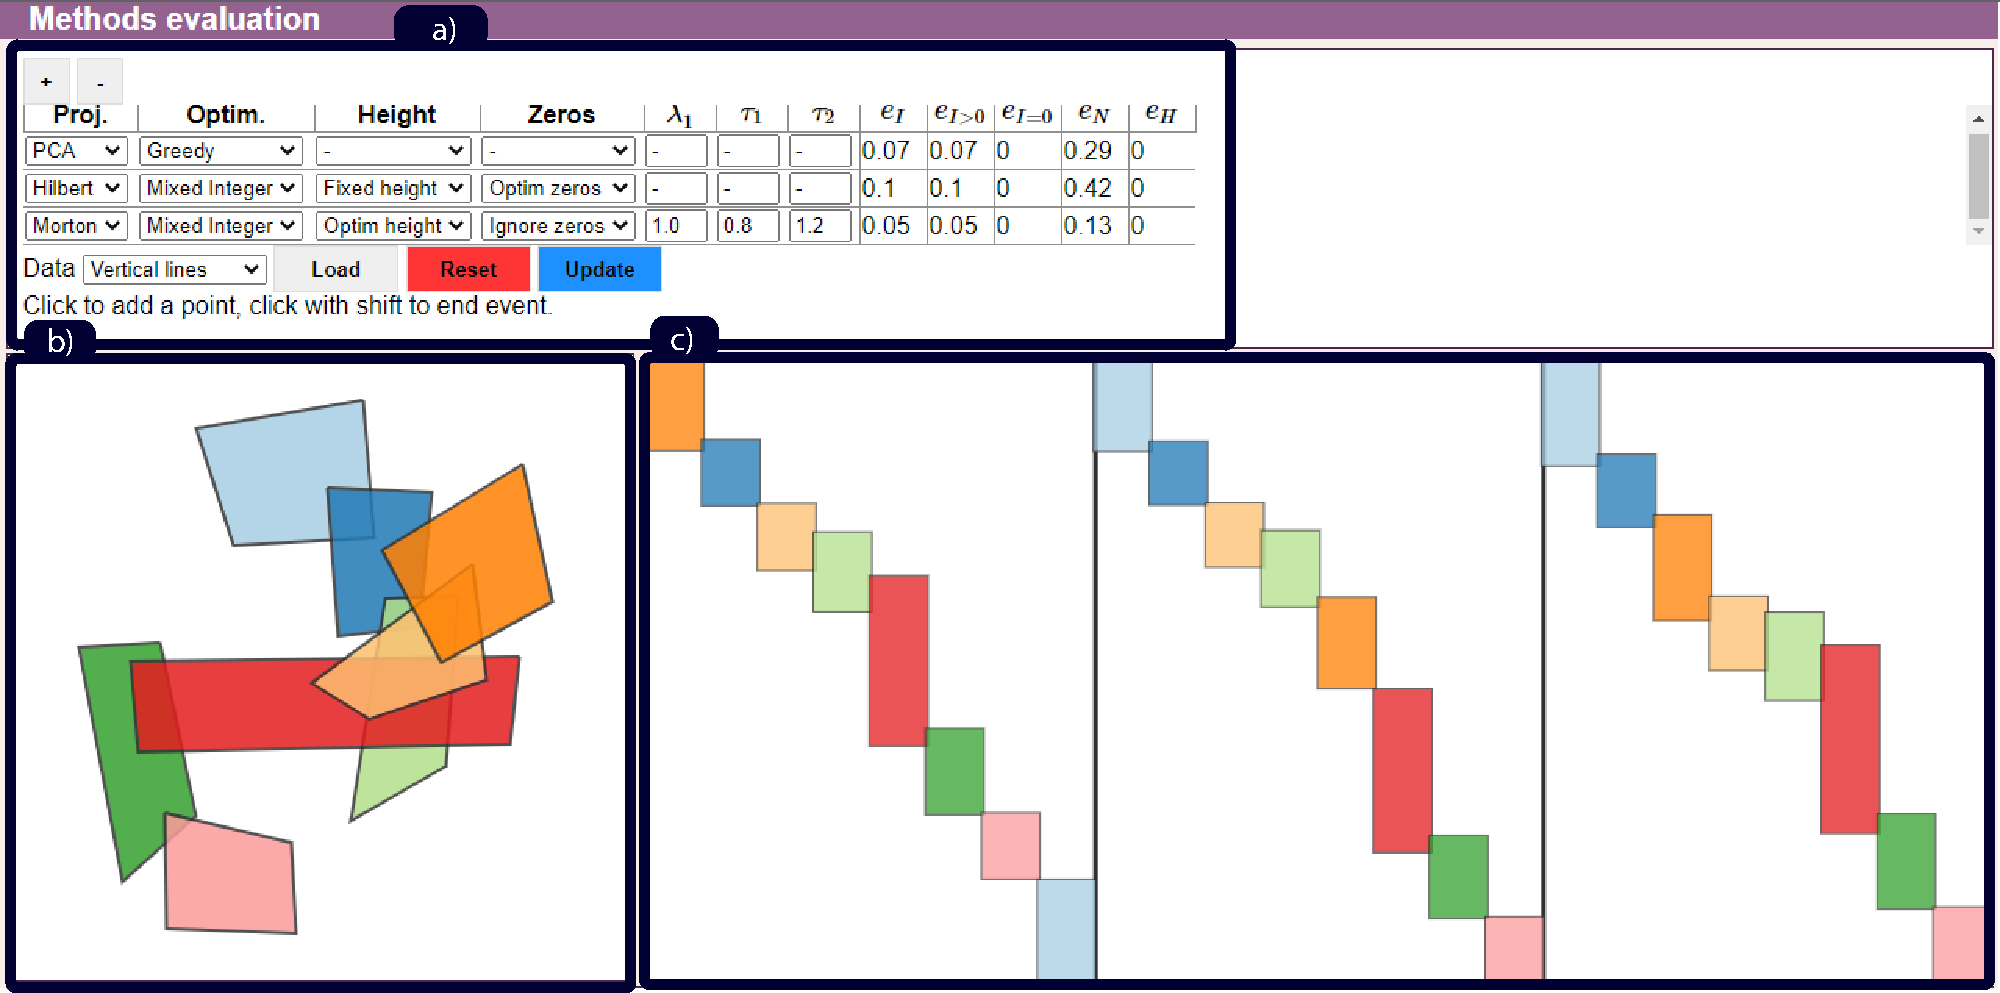
\includegraphics[width = \textwidth]{src/imgs/evaluation-tool.pdf}
    \caption{Source: Elaborated by author. The interface of the tool for the evaluation of different methods with generated datasets created by the user.}
    \label{fig:evaluation-tool}
\end{figure}

To facilitate the comparison between the projection and vertical positioning methods it was also implemented a tool for the analysis of the results for different datasets.
%
Using the same languages and libraries as the visualization tool, this interface can be divided into three panels as shown in Figure~\ref{fig:evaluation-tool}: a) a menu for the selection of the computed methods and information with the metrics for the respective methods, b) a panel where the user can draw events shapes with mouse clicks and c) a plot with the resulted visualization.
%
Below, not visible on the figure, there is also a panel with the mathematical description of the optimization methods.

%
This application permits the user to draw any set of events as convex polygons with mouse clicks, so it facilitates understanding the results and verifying hypotheses, 
%
however, it is a simplified version of the method,
%
the events are polygons, but it is not possible to represent the inner structure,
and it ignores the time information of events, 
%
so the final plot will have rectangles positioned horizontally in an arbitrary order and with fixed width.

On the top panel Fig.~\ref{fig:evaluation-tool} a), the user can select as many methods as they desire, there are two buttons with symbols \textit{+} and \textit{-} that respectively add a new method and remove the last method add.
%
Each method is represented in a row of the table, with the columns being the parameters and error metrics of the method.
%
In order, the parameters are the projection method (PCA, MDS, t-SNE, UMAP, Hilbert, Morton), the optimization method (greedy, convex), if the height will be optimized and if the intersections equal to $0$ will be considered, two options only necessary for the convex method, and the values for parameters $(\lambda, \tau_1, \tau_2)$ if the height will be optimized.
%
So if the user wants to use the greedy algorithm, it can select only the projection method and the optimization method, leaving the other values as default.

In the same table, there are also columns for the metrics, that will only appear after the plot is created.
%
In order, the metrics are the \textit{intersection error}, \textit{non-zero intersection error}, \textit{zero intersection error}, \textit{stress measure}, \textit{neighborhood error}, and \textit{height error}.

Below this table there are the controls for data selection, first, there is a selector to choose between a set of pre-determined datasets, that will be plotted by clicking on \textit{Load}.
%
The button \textit{Reset} is to delete all events drawn in the plot, and the button \textit{Update} is to make the information for the server, which will compute the resulting visualization and the metrics.

In Fig.~\ref{fig:evaluation-tool} b) is the panel for a plot of events that is interactive. When hovering this panel, a purple circle will appear, by clicking, the circle will be fixed, being the first point of the event, the user can create as many points a desire by clicking. To finish an event, the user must hold the \textit{shift} key, the purple circle will get darker, when clicking, the event is sent to the server, which will return the convex hull of points to substitute the circles. 
%
An example of this process is presented in Figure~\ref{fig:evaluation-tool-draw}.

\begin{figure}
    \centering
    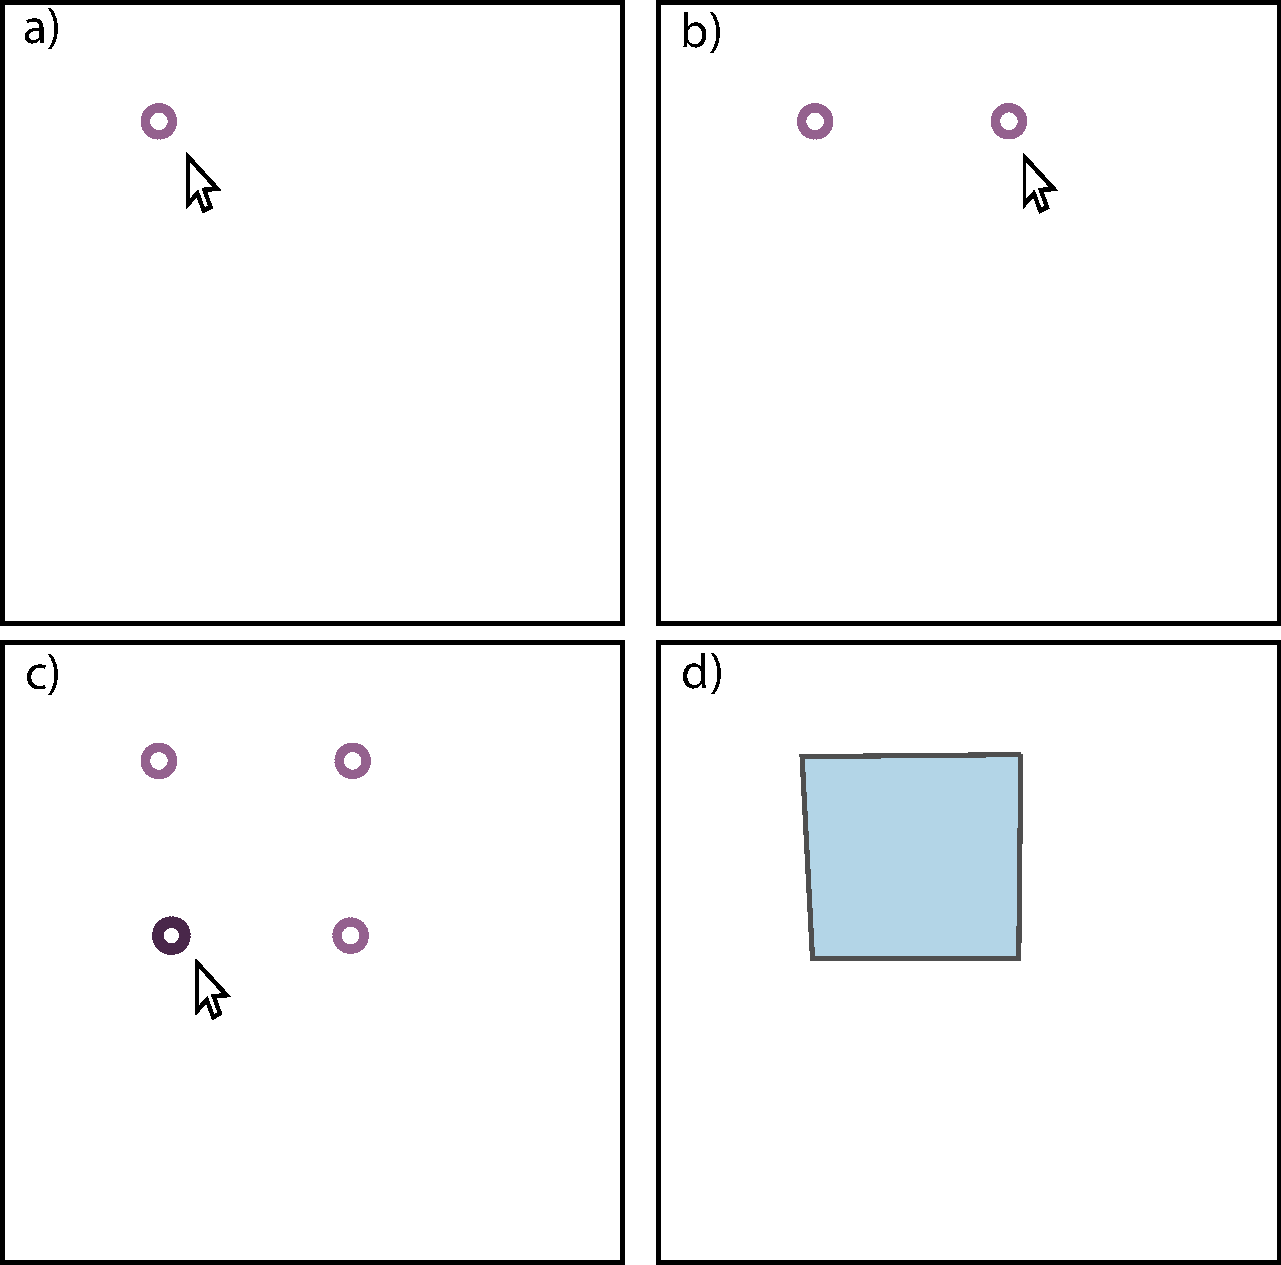
\includegraphics[width = 0.5\textwidth]{src/imgs/evaluation-tool-draw.pdf}
    \caption{Source: elaborated by author. An example process of creating a square event. On a) a purple circle is drawn under the cursor, on b) after a click, the first circle is fixed and another circle appears under the cursor, on c) three points are already fixed and when holding \textit{shift}, the circle under the cursor appears dark, on d) after clicking, the circles are substituted by the convex hull.}
    \label{fig:evaluation-tool-draw}
\end{figure}

After drawing a set of events, the user can click on \textit{Update} and it will be computed the vertical positioning algorithm, and the final plot will be shown in Fig.~\ref{fig:evaluation-tool-draw} c).
%
If there is more than one selected method, the plot will be divided in subplots of the same width, each subplot will have the result of a method. 
%
In the figure, three methods are selected, having three results.
%
The events are placed horizontally ordered by the y-position and with a fixed width to make them create small horizontal intersections just to be able to verify intersections.
